\documentclass{article}

\usepackage{etoolbox}       % toggle sections on or off
\newtoggle{draft}
\togglefalse{draft}
\newtoggle{arxiv}
\toggletrue{arxiv}

\iftoggle{draft}{
% WIP version
\usepackage{nips_2016}
}{
% Camera-ready version
\usepackage[final]{nips_2016}
}

\usepackage[utf8]{inputenc} % allow utf-8 input
\usepackage[T1]{fontenc}    % use 8-bit T1 fonts
\usepackage{hyperref}       % hyperlinks
\usepackage{url}            % simple URL typesetting
\usepackage{booktabs}       % professional-quality tables
\usepackage{amsfonts}       % blackboard math symbols
\usepackage{amsmath}        % split math environment, etc.
\usepackage{amsthm}         % theorems
\usepackage{graphicx}       % figures
\usepackage{nicefrac}       % compact symbols for 1/2, etc.
\usepackage{microtype}      % microtypography
\usepackage{tikz}           % diagrams
\usepackage{setspace}       % line spacing
\usepackage{subcaption}     % subfigures
\usepackage{xcolor}         % colors
\usepackage{algorithm}      % algorithm floating figures
\usepackage{algpseudocode}  % algorithm environment
\usepackage{algorithmicx}   % algorithm constructs
\usepackage{bm}             % mathbold symbols
\usepackage{url}            % urls

\usetikzlibrary{shapes,positioning}
\tikzset{>=latex}

\newtheorem{prop}{Proposition}
\newcommand\todo[1]{\textcolor{red}{TODO: #1}}
\newcommand{\bcom}[1]{{\leavevmode\color{blue}{[ben: #1]}}}
\newcommand{\EE}{\mathbb{E}}

\newcommand{\figureHeight}{5cm}

\renewcommand{\arraystretch}{1.3} % More space between table rows
\newcommand*\samethanks[1][\value{footnote}]{\footnotemark[#1]}

\def\algorithmautorefname{Algorithm}

\title{Adversarially Learned Inference}

% Using \And between authors leaves it to LaTeX to determine where to
% break the lines. Using \AND forces a line break at that point. So,
% if LaTeX puts 3 of 4 authors names on the first line, and the last
% on the second line, try using \AND instead of \And before the third
% author name.

\author{
    Vincent Dumoulin\thanks{MILA, Université de Montréal} \\
    \texttt{vincent.dumoulin@umontreal.ca} \\
    \And
    Ishmael Belghazi\samethanks[1] \\
    \texttt{ishmael.belghazi@gmail.com} \\
    \And
    Ben Poole \thanks{Neural Dynamics and Computation Lab, Stanford} \\
    \texttt{poole@cs.stanford.edu} \\
    \And
    Alex Lamb\samethanks[1] \\
    \texttt{alex6200@gmail.com} \\
    \And
    Martin Arjovsky\samethanks[1] \\
    \texttt{martinarjovsky@gmail.com} \\
    \And
    Olivier Mastropietro\samethanks[1] \\
    \texttt{oli.mastro@gmail.com} \\
    \And
    Aaron Courville\samethanks[1]\textnormal{,\ \ CIFAR Fellow} \\
    \texttt{aaron.courville@gmail.com} \\
}

\begin{document}

\maketitle

\begin{abstract}
We introduce the adversarially learned inference (ALI) model, which jointly
learns a generation network and an inference network using an adversarial
process. The generation network maps samples from stochastic latent variables
to the data space while the inference network maps training examples in data
space to the space of latent variables. An adversarial game is cast between
these two networks and a discriminative network that is trained to distinguish
between joint latent/data-space samples from the generative network and joint
samples from the inference network.  We illustrate the ability of the model to learn mutually
coherent inference and generation networks through the inspections of model
samples and reconstructions and confirm the usefulness of the learned
representations by obtaining state-of-the-art on the semi-supervised SVHN
task, beating both DCGAN and VAE.
\end{abstract}

\section{Introduction}

Deep directed generative models have emerged as a powerful technique for
modeling complex high-dimensional datasets. These models permit fast ancestral
sampling, but are often challenging to learn due to the complexities of
inference. Recently, two classes of algorithms have emerged as effective for
learning deep directed generative models: 1) Techniques based on the
Variational Autoencoder (VAE) that aim to improve the quality and efficiency of
inference by learning an inference
machine~\citep{kingma2013auto,rezende2014stochastic}, and 2) techniques based
on Generative Adversarial Networks (GANs) that bypass inference
altogether~\citep{goodfellow2014generative}. While both techniques are provably
consistent given infinite capacity and data, they learn very different
generative models on typical datasets.

VAE-based techniques aim to maximize the log-likelihood of the observed data
$\bm{x}$ by introducing a set of stochastic latent variables $\bm{z}$ and
marginalizing them out of the joint distribution $p(\bm{x}, \bm{z})$. While
exact marginalization of the latent variables is generally intractable, the VAE
introduces an approximate posterior $q(\bm{z} \mid \bm{x})$ and maximizes a
variational lower bound on the log-likelihood of $p(\bm{x})$. Several VAE
variants have been proposed. One approach improves the quality of the
approximate posterior using hybrid Monte Carlo \citep{salimans2014markov}.
Another approach, known as the DRAW model \citep{gregor2015draw}, subdivides
the inference and generation processes into multiple sequential steps through
the use of recurrent neural networks and an attention mechanism.

Despite the impressive progress of VAE-based approaches for learning deep
directed generative models, they still suffer from a well-recognized issue of
the maximum likelihood training paradigm. Models trained to maximize likelihood
of the training data tend to be conservative, distributing probability mass
diffusely over the data space~\citep{Theis2015}. In the case of learning
generative models of images, this results in almost all probability mass lying
outside the relatively restrictive subset of pixel space occupied by natural
images. The direct consequence of this is that image samples from VAE-trained
models tend to be
blurry~\citep{goodfellow2014generative,larsen2015autoencoding}.

On the other hand, GAN-based techniques are trained via an adversarial process
that does not appear to suffer from the same probability mass diffusion problem
as does maximum likelihood. In the GAN paradigm, a discriminative network is
trained to distinguish between the empirical distribution and samples produced
by a generative network. Meanwhile, the generative network is trained to
produce samples intended to fool the discriminator into classifying them as
true samples from the training set.  While the adversarial setting presents a
challenging (and often unstable) training paradigm, it results in a generative
network capable of producing samples that exceed those of the best VAE
techniques~\citep{radford2015unsupervised,larsen2015autoencoding}. Recent
GAN-based convolutional generative networks have been able to achieve dramatic
improvements in the quality of synthetic
images~\citep{radford2015unsupervised,denton2015deep}.

While GANs learn a generative model that produces higher-quality samples, only
the VAE-based models learn an efficient mechanism for inference. For
applications such as semi-supervised learning, GANs are insufficient as they do
not provide an efficient inference mechanism.  Recently, efforts have aimed to
bridge the gap between VAEs and GANs, to learn generative models with
higher-quality samples while learning an efficient inference
network~\citep{larsen2015autoencoding,lamb2016discriminative,
dosovitskiy2016generating}. While this is certainly a promising research
direction, VAE-GAN hybrids tend to manifest a compromise of the strengths and
weaknesses of both approaches.

In this paper, we propose a novel approach  to integrate efficient inference
with the GAN framework. Our approach, called Adversarially Learned Inference
(ALI), casts the learning of both an inference machine (or encoder) and a deep
directed generative model (or decoder) in an GAN-like adversarial framework. A
discriminator is trained to discriminate joint samples of the data and the
corresponding latent variable from the encoder (or approximate posterior) from
joint samples from the decoder. In opposition to the discriminator, we have two
generative models, the encoder and the decoder, trained together to fool the
discriminator.

GAN is an example of how one can leverage highly effective discriminative
training techniques in service of learning deep generative networks. Here, we
are effectively doubling down on the gambit that we can exploit discriminative
training. Not only are we asking the discriminator to distinguish synthetic
samples from real data, but we are requiring it to distinguish between two
joint distributions over the data space and the latent variables.

With experiments on a toy task, the Street View House Numbers (SVHN) dataset
\citep{netzer2011reading}, the CIFAR-10 object recognition dataset \citep{krizhevsky2009learning}, the
CelebA face dataset~\citep{liu2015deep} and a downsampled version of the
ImageNet dataset~\citep{russakovsky2015imagenet}, we show qualitatively that we
maintain the high sample fidelity associated with the GAN framework, while
gaining the ability to perform efficient inference.

\section{Adversarially learned inference}

\begin{figure}[t]
    \centering
    \begin{tikzpicture}[remember picture,node distance=2cm,
                        box/.style={draw,rectangle,rounded corners}]
        \node[box,rectangle] (q) {
            \begin{tikzpicture}
                \node (x) {$\bm{x} \sim q(\bm{x})$};
                \node[above=of x]
                    (z_hat) {$\hat{\bm{z}} \sim q(\bm{z} \mid \bm{x})$};
            \end{tikzpicture}
        };
        \node[box,minimum height=1cm,minimum width=2cm,right=of q]
            (discriminator) {$D(\bm{x}, \bm{z})$};
        \node[box,right= of discriminator] (p) {
            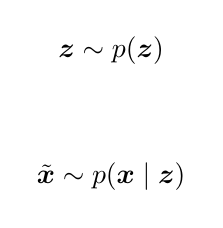
\begin{tikzpicture}
                \node (x_tilde) {$\tilde{\bm{x}} \sim p(\bm{x} \mid \bm{z})$};
                \node[above=of x_tilde] (z) {$\bm{z} \sim p(\bm{z})$};
            \end{tikzpicture}
        };
        \draw[->] (x) -- (z_hat) node[midway,above,rotate=90]
			{$\scriptstyle G_z(\bm{x})$};
        \draw[->] (z) -- (x_tilde) node[midway,above,rotate=270]
			{$\scriptstyle G_x(\bm{z})$};
        \draw[->] (q) -- (discriminator) node[midway,above]
			{$(\bm{x}, \hat{\bm{z}})$};
        \draw[->] (p) -- (discriminator) node[midway,above]
			{$(\tilde{\bm{x}}, \bm{z})$};
    \end{tikzpicture}
    \caption{\label{fig:model} The adversarially learned inference (ALI) game.}
\end{figure}

Consider the two following probability distributions over $\bm{x}$ and $\bm{z}$:
\begin{itemize}
    \item the \emph{encoder} joint distribution
		$q(\bm{x}, \bm{z}) = q(\bm{x}) q(\bm{z} \mid \bm{x})$,
    \item the \emph{decoder} joint distribution
		$p(\bm{x}, \bm{z}) = p(\bm{z}) p(\bm{x} \mid \bm{z})$.
\end{itemize}
These two distributions have marginals that are known to us: the encoder
marginal $q(\bm{x})$ is the empirical data distribution and the decoder
marginal $p(\bm{z})$ is usually defined to be a simple, factorized
distribution, such as the standard Normal distribution $p(\bm{z}) =
\mathcal{N}(\bm{0},\bm{I})$. As such, the generative process between $q(\bm{x},
\bm{z})$ and $p(\bm{x}, \bm{z})$ is reversed.

ALI's objective is to match the two joint distributions. If this is achieved,
then we are ensured that all marginals match and all conditional distributions
also match. In particular, we are assured that the conditional $q(\bm{z} \mid
\bm{x})$ matches the posterior $q(\bm{z} \mid \bm{x})$.

In order to match the joint distributions, an adversarial game is played. Joint
pairs $(\bm{x}, \bm{z})$ are drawn either from $q(\bm{x}, \bm{z})$ or
$p(\bm{x}, \bm{z})$, and a discriminator network learns to discriminate between
the two, while the encoder and decoder networks are trained to fool the
discriminator.

The value function describing the game is given by:
\begin{equation}
\label{eq:value_function}
\begin{split}
    \min_G \max_D V(D, G)
	&= \mathbb{E}_{q(\bm{x})}[\log(D(\bm{x}, G_z(\bm{x})))]
	 + \mathbb{E}_{p(\bm{z})}[\log(1 - D(G_x(\bm{z}), \bm{z}))] \\
    &= \iint q(\bm{x}) q(\bm{z} \mid \bm{x})
		     \log(D(\bm{x}, \bm{z})) d\bm{x} d\bm{z} \\
    &+ \iint p(\bm{z}) p(\bm{x} \mid \bm{z})
			 \log(1 - D(\bm{x}, \bm{z})) d\bm{x} d\bm{z}.
\end{split}
\end{equation}

Sampling from $q(\bm{z} \mid \bm{x})$ amounts to drawing an $\bm{x}$ from the
data distribution and propagating the sample through the encoder network
$\left(\bm{\mu}_z,\bm{\sigma}_z\right) = G_z(\bm{x})$, then generating
$\hat{\bm{z}} \sim \mathcal{N}\left(\bm{\mu}_z,\bm{\sigma}_z\right)$. Sampling
from $p(\bm{x} \mid \bm{z})$ amounts to sampling from $p(\bm{z}) =
\mathcal{N}\left(\bm{0},\bm{I}\right)$ and propagating the sample through the
decoder network to recover $\tilde{\bm{x}}$.

The discriminator is trained to distinguish between samples from the encoder
$(\bm{x},\hat{\bm{z}}) \sim q(\bm{x}, \bm{z})$ and samples from the decoder
$(\tilde{\bm{x}}, \bm{z}) \sim p(\bm{x},\bm{z})$. The generator is trained to
fool the discriminator, i.e., to generate $\bm{x}, \bm{z}$ pairs from
$q(\bm{x},\bm{z})$ or $p(\bm{x}, \bm{z})$ that are indistinguishable one from
another. See \autoref{fig:model} for a diagram of the adversarial game and
\autoref{alg:ali} for an algorithmic description of the procedure.

In such a setting, and under the assumption of an optimal discriminator, the
generator minimizes the Jensen-Shannon divergence \citep{lin1991divergence}
between $q(\bm{x}, \bm{z})$ and $p(\bm{x}, \bm{z})$. This can be shown using
the same proof sketch as in the original GAN
paper~\citep{goodfellow2014generative}.

\begin{algorithm}[t]
\setstretch{1.35}
\begin{algorithmic}
    \State $\theta_{g}, \theta_{d} \gets \text{initialize network parameters}$
    \Repeat
		\State $\bm{x}^{(1)}, \ldots, \bm{x}^{(M)} \sim q(\bm{x})$
            \Comment{Draw $M$ samples from the dataset and the prior}
		\State $\bm{z}^{(1)}, \ldots, \bm{z}^{(M)} \sim p(\bm{z})$
		\State $\hat{\bm{z}}^{(i)} \sim q(\bm{z} \mid \bm{x} = \bm{x}^{(i)}),
			    \quad i = 1, \ldots, M$
            \Comment{Sample from the conditionals}
		\State $\tilde{\bm{x}}^{(j)} \sim p(\bm{x} \mid \bm{z} = \bm{z}^{(j)}),
				\quad j = 1, \ldots, M$
        \State $\rho_q^{(i)} \gets D(\bm{x}^{(i)}, \hat{\bm{z}}^{(i)}),
				\quad i = 1, \ldots, M$
            \Comment{Compute discriminator predictions}
        \State $\rho_p^{(j)} \gets D(\tilde{\bm{x}}^{(j)}, \bm{z}^{(j)}),
				\quad j = 1, \ldots, M$
        \State $\mathcal{L}_d \gets
            -\frac{1}{M} \sum_{i=1}^M \log(\rho_q^{(i)})
            -\frac{1}{M} \sum_{j=1}^M\ log(1 - \rho_p^{(j)})$
            \Comment{Compute discriminator loss}
        \State $\mathcal{L}_g \gets
            -\frac{1}{M} \sum_{i=1}^M \log(1 - \rho_q^{(i)})
            -\frac{1}{M} \sum_{j=1}^M \log(\rho_p^{(j)})$
            \Comment{Compute generator loss}
        \State $\theta_d \gets \theta_d - \nabla_{\theta_d} \mathcal{L}_d$
            \Comment{Gradient update on discriminator network}
        \State $\theta_g \gets \theta_g - \nabla_{\theta_g} \mathcal{L}_g$
            \Comment{Gradient update on generator networks}
    \Until{convergence}
\end{algorithmic}
\caption{\label{alg:ali} The ALI training procedure.}
\end{algorithm}

\subsection{Relation to GAN}
ALI bears close resemblance to GAN, but it differs from it in the two following
ways:

\begin{itemize}
	\item The generator has two components: the encoder, $G_z(\bm{x})$, which
		maps data samples $\bm{x}$ to $\bm{z}$-space, and the decoder
		$G_x(\bm{z})$, which maps samples from the prior $p(\bm{z})$ (a source
		of noise) to the input space.
	\item The discriminator is trained to distinguish between joint pairs
		$(\bm{x}, \hat{\bm{z}} = G_x(\bm{x}))$ and $(\tilde{\bm{x}} =
		G_x(\bm{z}), \bm{z})$, as opposed to marginal samples $\bm{x} \sim
		q(\bm{x})$ and $\tilde{\bm{x}} \sim p(\bm{x})$.
\end{itemize}


\subsection{Reparametrization trick}
In order for the gradient to propagate from the discriminator network to the
encoder and decoder networks, the gradient needs to flow through the sampling
processes $\hat{\bm{z}} \sim q(\bm{z} \mid \bm{x})$ and $\tilde{\bm{x}} \sim
p(\bm{x} \mid \bm{z})$.

To achieve this, the reparametrization trick
\citep{kingma2013fast,bengio2013deep,bengio2013estimating} is employed. Instead
of sampling directly from the desired distribution, the random variable is
computed as a deterministic transformation of some noise such that its
distribution is the desired distribution.

For instance, if $q(z \mid x) = \mathcal{N}(\mu(x), \sigma^2(x)I)$, one can
draw samples by computing

\begin{equation}
    z = \mu(x) + \sigma(x) \odot \epsilon, \quad
    \epsilon \sim \mathcal{N}(0, I).
\end{equation}

\subsection{Generator value function}

As with GANs, when ALI's discriminator gets too far ahead, its generator may
have a hard time minimizing the value function in \autoref{eq:value_function}.
If the discriminator's output is sigmoidal, then the gradient of the value
function with respect to the discriminator's output vanishes to zero as the
output saturates.

As a workaround, the generator is trained to maximize
\begin{equation}
\label{eq:generator_value_function}
    V'(D, G) = \mathbb{E}_{q(\bm{x})}[\log(1 - D(\bm{x}, G_{\bm{z}}(\bm{x})))] +
               \mathbb{E}_{p(\bm{z})}[\log(D(G_{\bm{x}}(\bm{z}), \bm{z}))] \\
\end{equation}
which has the same fixed points but whose gradient is stronger when the
discriminator's output saturates.

The adversarial game does not require an analytical expression for the joint
distributions. This means we can introduce variable changes without having to
know the explicit distribution over the new variable.  For instance, sampling
from $p(z)$ could be done by sampling $\epsilon \sim \mathcal{N}(0, I)$ and
passing it through an arbitrary differentiable function $z = f(\epsilon)$.

However, gradient propagation into the encoder and decoder networks relies on
the reparametrization trick, which means that ALI is not directly
applicable to either applications with discrete data or to models with
discrete latent variables.

\begin{figure}[p]
    \centering
    \begin{subfigure}[t]{0.49\textwidth}
        \centering
        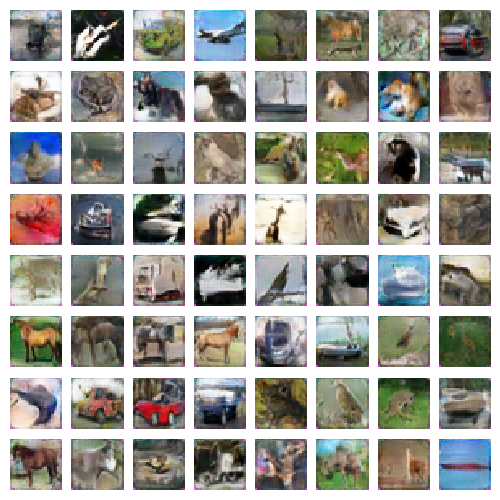
\includegraphics[height=\figureHeight]{cifar10_samples.png}
        \caption{\label{fig:cifar10_samples} CIFAR10 samples.}
    \end{subfigure}
    \hfill
    \begin{subfigure}[t]{0.49\textwidth}
        \centering
        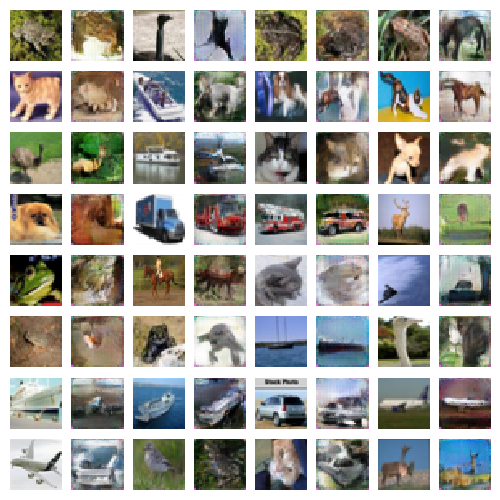
\includegraphics[height=\figureHeight]{cifar10_reconstructions.png}
        \caption{\label{fig:cifar10_reconstructions} CIFAR10
          reconstructions.}
    \end{subfigure}
    \caption{\label{fig:cifar10_images} Samples and reconstructions on the
        CIFAR10 dataset. For the reconstructions, odd columns are
        original samples from the validation set and even columns are
        corresponding reconstructions (e.g., second column contains
        reconstructions of the first column's validation set samples).}
\end{figure}

\begin{figure}[p]
    \centering
    \begin{subfigure}[t]{0.49\textwidth}
        \centering
        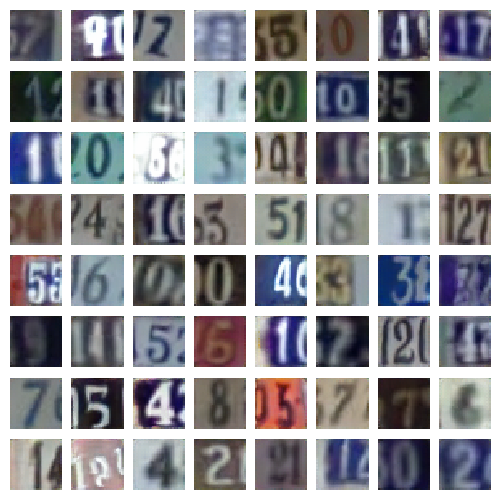
\includegraphics[height=\figureHeight]{svhn_samples.png}
        \caption{\label{fig:svhn_samples} SVHN samples.}
    \end{subfigure}
    \hfill
    \begin{subfigure}[t]{0.49\textwidth}
        \centering
        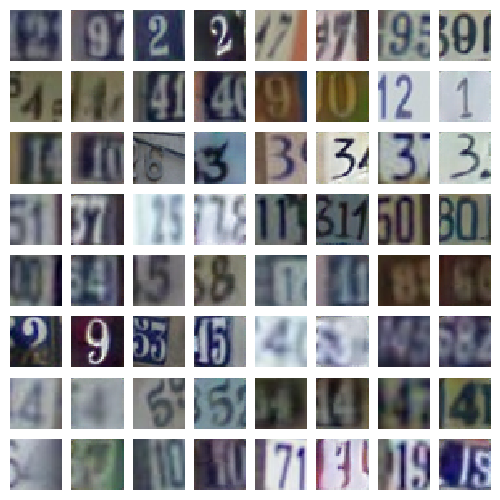
\includegraphics[height=\figureHeight]{svhn_reconstructions.png}
        \caption{\label{fig:svhn_reconstructions} SVHN reconstructions.}
    \end{subfigure}
    \caption{\label{fig:svhn_images} Samples and reconstructions on the SVHN
        dataset. For the reconstructions, odd columns are
        original samples from the validation set and even columns are
        corresponding reconstructions.}
\end{figure}

\begin{figure}[p]
    \centering
    \begin{subfigure}[t]{0.49\textwidth}
        \centering
        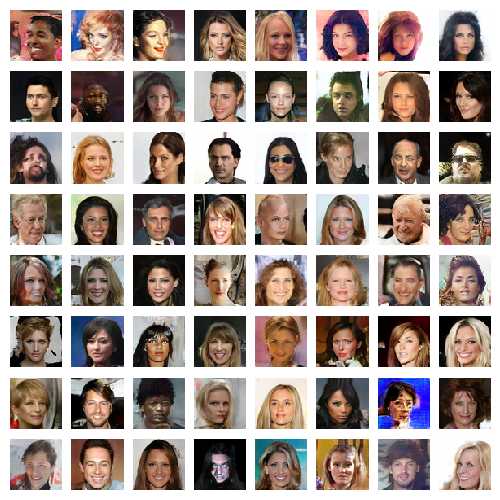
\includegraphics[height=\figureHeight]{celeba_samples.png}
        \caption{\label{fig:celeba_samples} CelebA samples.}
    \end{subfigure}
    \hfill
    \begin{subfigure}[t]{0.49\textwidth}
        \centering
        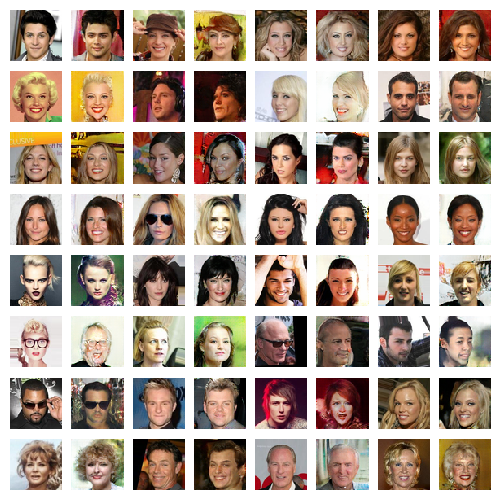
\includegraphics[height=\figureHeight]{celeba_reconstructions.png}
        \caption{\label{fig:celeba_reconstructions} CelebA reconstructions.}
    \end{subfigure}
    \caption{\label{fig:celeba_images} Samples and reconstructions on the CelebA
        dataset. For the reconstructions, odd columns are
        original samples from the validation set and even columns are
        corresponding reconstructions.}
\end{figure}

\subsection{Discriminator optimality}
\label{sec:disc_opt}
\begin{prop}
    Given a fixed generator $G$, the optimal discriminator is given by
    \begin{equation}
    \label{eq:optgansol}
		D^*(x, z) = \frac{q(x, z)}{q(x, z) + p(x, z)}.
    \end{equation}
\end{prop}
\begin{proof}
	For a fixed generator $G$, the complete data value function is
	\begin{equation}
	\label{eq:cdganvalue}
		V(D, G) = \EE_{x,z \sim q(x,z)}[\log(D(x, z))]
		        + \EE_{x, z \sim p(x, z)}[\log(1 - D(x, z))].
	\end{equation}
	The result follows by the concavity of the log and the simplified
	Euler-Lagrange equation first order conditions on
	$(x, z) \rightarrow D(x, z)$.
\end{proof}

\subsection{Relationship with the Jensen-Shannon divergence}
\label{sec:jsd_rel}
\begin{prop}
	Under an optimal discriminator $D^{*}$, the generator minimizes the
	Jensen-Shanon divergence which attains its minimum if and only if
	$q(\bm{x}, \bm{z}) = p(\bm{x}, \bm{z})$.
\end{prop}
\begin{proof}
	The proof is a straightforward extension of the proof
	in~\cite{goodfellow2014generative}.
\end{proof}

\subsection{Multilayer extensions of ALI}
It is straightforward to extend the ALI framework to multiple stochastic layers,
i.e.,
\begin{align}
    p(\bm{x}, \bm{z}_1,\bm{z}_2,\dots,\bm{z}_L) &= p(\bm{z}_L) p(\bm{z}_{L-1}
    \mid \bm{z}_L) \cdots p(\bm{z}_{1} \mid \bm{z}_2, \dots, \bm{z}_L)
    p(\bm{x} \mid \bm{z}_1, \dots, \bm{z}_L) \\
    q(\bm{x}, \bm{z}_1,\bm{z}_2,\dots,\bm{z}_L) &= q(\bm{x}) p(\bm{z}_{1}
    \mid \bm{x}) p(\bm{z}_{2} \mid \bm{z}_1, \bm{x}) \cdots
    p(\bm{z}_{L} \mid \bm{z}_1, \dots, \bm{z}_{L-1}, \bm{x}).
\end{align}
In this case, the discriminator takes as input either $(\bm{x},
\hat{\mathbf{z}}_{1:L}) \sim q(\bm{x}, \mathbf{z}_{1:L})$ or $(\tilde{\bm{x}},
\mathbf{z}_{1:L}) \sim p(\bm{x}, \mathbf{z}_{1:L})$ and tries to determine
which joint the samples were drawn from. The generator trains the distributions
$q(\mathbf{z}_{1:L} \mid \bm{x})$, $p(\mathbf{z}_{1:L})$ and $p(\bm{x} \mid
\mathbf{z}_{1:L})$ to fool the discriminator.

\section{Related Work}

Other recent papers explore hybrid approaches to generative modelling. One such
approach is to relax the probabilistic interpretation of the VAE model by
replacing either the KL-divergence term or the reconstruction term with
variants that have better properties. The adversarial autoencoder model
\citep{makhzani2015adversarial} replaces the KL-divergence term with a
discriminator that is trained to distinguish between approximate posterior and
prior samples, which provides a more flexible approach to matching the marginal
$q(\bm{z})$ and the prior. Other papers explore replacing the reconstruction
term with either GANs or auxiliary networks. \citet{larsen2015autoencoding}
collapse the decoder of a VAE and the generator of a GAN into one network in
order to supplement the reconstruction loss with a learned similarity metric.
\citet{lamb2016discriminative} use the hidden layers of a pre-trained
classifier as auxiliary reconstruction losses to help the VAE focus on
higher-level details when reconstructing. \citet{dosovitskiy2016generating}
combine both ideas into a unified loss function.

ALI's approach is also reminiscent of the adversarial autoencoder model, which
employs a GAN to distinguish between samples from the approximate posterior
distribution $q(\bm{z} \mid \bm{x})$ and prior samples. However, unlike
adversarial autoencoders, no explicit reconstruction loss is being optimized in
ALI, and the discriminator receives joint pairs of samples $(\bm{x}, \bm{z})$
rather than marginal $\bm{z}$ samples.

\section{Experimental results}

\begin{figure}[t]
    \centering
    \begin{subfigure}[t]{0.49\textwidth}
        \centering
        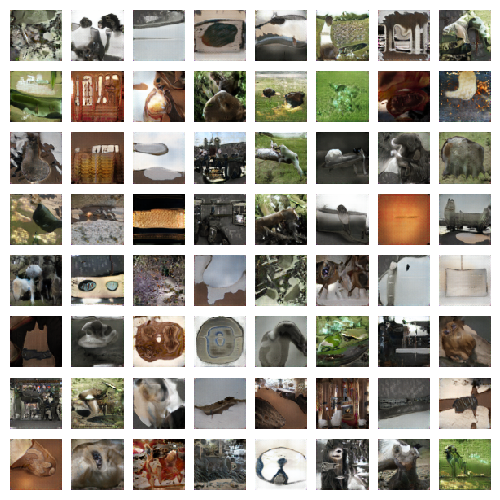
\includegraphics[height=\figureHeight]{tiny_imagenet_samples.png}
        \caption{\label{fig:tiny_imagenet_samples} Tiny ImageNet samples.}
    \end{subfigure}
    \hfill
    \begin{subfigure}[t]{0.49\textwidth}
        \centering
        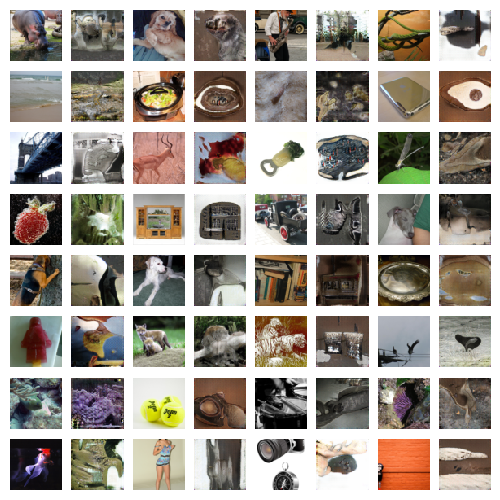
\includegraphics[height=\figureHeight]{tiny_imagenet_reconstructions.png}
        \caption{\label{fig:tiny_imagenet_reconstructions} Tiny ImageNet
            reconstructions.}
    \end{subfigure}
    \caption{\label{fig:tiny_imagenet_images} Samples and reconstructions on the
        Tiny ImageNet dataset. For the reconstructions, odd columns are original
        samples from the validation set and even columns are corresponding
        reconstructions.}
\end{figure}

\begin{table}[t]
\centering
\begin{tabular}{@{}llll@{}} \toprule
Method                                         & Error rate                      \\ \midrule
KNN (as reported in \citet{zhao2015stacked})   & $77.93\%$                       \\
TSVM \citep{vapnik1998}                        & $66.55\%$                       \\
VAE (M1 + M2) \citep{kingma2014semi}           & $36.02\%$                       \\
SWWAE without dropout \citep{zhao2015stacked}  & $27.83\%$                       \\
SWWAE with dropout \citep{zhao2015stacked}     & $23.56\%$                       \\
DCGAN + L2-SVM \citep{radford2015unsupervised} & $22.18\% (\pm 1.13\%)$          \\ \midrule
ALI (ours)                                     & $\mathbf{19.14\% (\pm 0.50\%)}$ \\
\bottomrule
\end{tabular}
\vspace{0.2cm}
\caption{\label{tab:semi-supervised} SVHN test set error rates for
	semi-supervised learning. 1000 training examples were used.}
\end{table}

We applied ALI to four different datasets, namely CIFAR10
\citep{krizhevsky2009learning}, SVHN \citep{netzer2011reading}, CelebA
\citep{liu2015deep} and a center-cropped, $64 \times 64$ version if the ImageNet
dataset \citep{russakovsky2015imagenet}.\footnote{
    The code for all experiments can be found at
    \url{https://github.com/IshmaelBelghazi/ALI}. Readers can also consult the
    accompanying website at \url{https://ishmaelbelghazi.github.io/ALI}.}

In addition to these larger scale experiments, we were interested in studying
how modeling the joint distribution impacted ALI in its ability to capture the
underlying data density. To this end, we applied ALI to a 2-D synthetic
dataset.

The use of batch normalization \citep{ioffe2015batch} in all layers (except the
output layer) of $G_z(\bm{x})$ and $G_x(\bm{z})$ was crucial to the generator's
success in fooling the discriminator. We also found that in order to stabilize
training, batch normalization should not be applied in layers of the
discriminator which are influenced by $\bm{z}$.

Transposed convolutions are used in $G_x(\bm{z})$. This operation corresponds
to the transpose of the matrix representation of a convolution, i.e., the
gradient of the convolution with respect to its inputs. For more details about
transposed convolutions, see \citet{dumoulin2016guide}.

\subsection{Samples}
For each dataset, samples are presented (Figures \ref{fig:cifar10_samples},
\ref{fig:svhn_samples}, \ref{fig:celeba_samples} and
\ref{fig:tiny_imagenet_samples}). They exhibit the same image fidelity as samples
from other adversarially-trained models.

\subsection{Reconstructions}
We also qualitatively evaluate the fit between the conditional distribution
$q(\bm{z} \mid \bm{x})$ and the posterior distribution $p(\bm{z} \mid \bm{x})$
by sampling $\hat{\bm{z}} \sim q(\bm{z} \mid \bm{x})$ and $\hat{\bm{x}} \sim
p(\bm{x} \mid \bm{z} = \hat{\bm{z}})$ (Figures
\ref{fig:cifar10_reconstructions}, \ref{fig:svhn_reconstructions},
\ref{fig:celeba_reconstructions} and \ref{fig:tiny_imagenet_reconstructions}).
This corresponds to reconstructing the input in a VAE setting. Interestingly,
even though reconstruction quality is not explictly enforced in the objective
function, the trained models achieve good reconstruction in practice, which
suggests that the conditional $q(\bm{z} \mid \bm{x})$ is indeed a good
approximation of the posterior $p(\bm{z} \mid \bm{x})$.

Reconstructions in ALI are quite different from reconstructions in
VAE-like models. Instead of focusing on achieving a pixel-perfect
reconstruction, ALI produces reconstructions that often faithfully
represent more abstract features of the input images, while   
 making mistakes in capturing exact object placement, color, style and
(in extreme cases) object identity. These reconstructions suggest that the
ALI latent variable representations are potentially more invariant to these less
interesting factors of variation in the input and do not devote model
capacity to capturing these factors.

\subsection{Semi-supervised learning}
The fact that ALI's latent representation tends to focus on semantic
information at the expense of low-level details leads us to believe that
ALI may be well suited to semi-supervised tasks. We empirically verify this
by achieving state of the art on the semi-supervised SVHN classification task.
Results are presented in \autoref{tab:semi-supervised}.

We follow the procedure outlined by \citet{radford2015unsupervised}. We train an
L2-SVM on the learned representations of a model trained on SVHN. The last three
hidden layers of the encoder as well as its output are concatenated to form a
8960-dimensional feature vector. A 10,000 example held-out validation set is
taken from the training set and is used for model selection. The SVM is trained
on 1000 examples taken at random from the remainder of the training set. The
test error rate is measured for 100 different SVMs trained on different random
1000-example training sets, and the average error rate is measured along with
its standard deviation.

\subsection{Comparison with GAN on a toy task}

Figure \ref{fig:mixture} shows a comparison of the ability of GAN and ALI to fit
a simple 2-dimensional synthetic gaussian mixture dataset. The decoder and
discriminator networks are matched between ALI and GAN, and the hyperparameters
are the same. In this experiment, ALI converges faster than GAN and to a better
solution.  Despite the relative simplicity of the data distribution, GAN
partially failed to converge to the distribution, ignoring the central mode.

The toy task also exhibits nice properties of the features learned by ALI: when
mapped to the latent space, data samples cover the whole prior, and they get
clustered by mixture components, with a clear separation between each mode.

\begin{figure}[t]
    \centering
    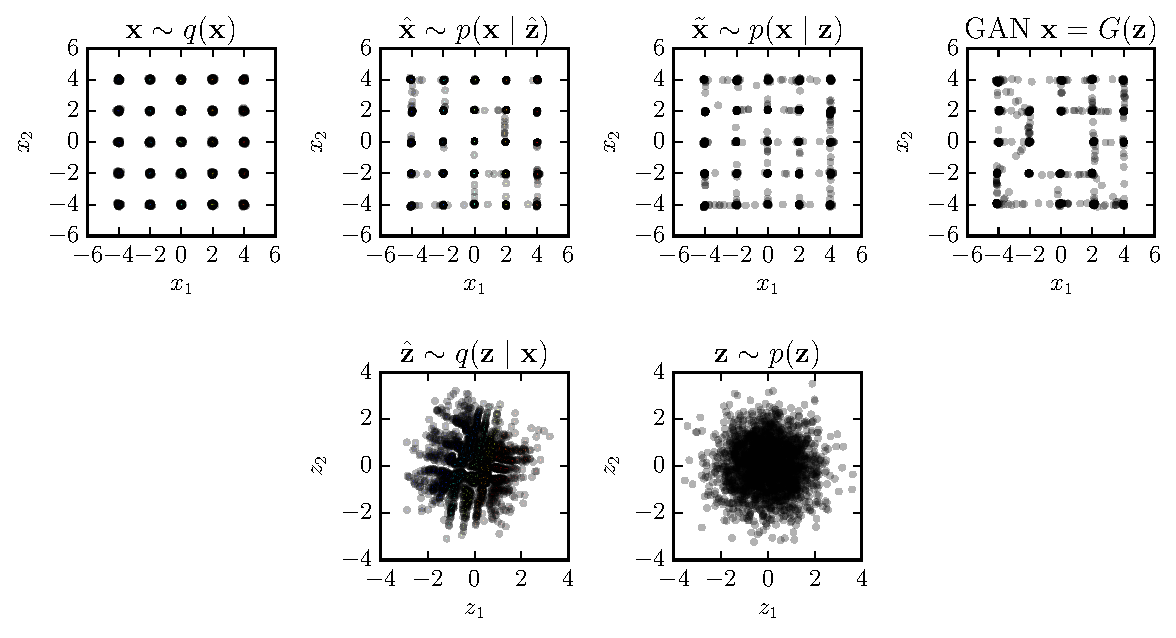
\includegraphics[width=\textwidth]{mixture_plot.pdf}
    \caption{\label{fig:mixture} Comparison of ALI and GAN on a synthetic
      gaussian mixture dataset. In the top row, from left to right: data
      samples, ALI reconstructions, ALI samples, GAN samples. In the bottom row,
      from left to right: ALI encodings, prior samples. The nine mixture modes,
      their ALI encodings and their ALI reconstructions have been color-coded
      to facilitate visualization.}
\end{figure}

\section{Conclusion}

We introduced the adversarially learned inference (ALI) model, which jointly
learns a generation network and an inference network using an adversarial
process. The model learns mutually coherent inference and generation networks,
as exhibited by its reconstructions. The induced latent variable mapping is
shown to be useful, achieving state-of-the-art results on semi-supervised SVHN
house number classification, beating both DCGAN and VAE.

\iftoggle{draft}{}{%
\subsubsection*{Acknowledgments}

The authors would like to acknowledge the support of the following agencies for
research funding and computing support: NSERC, Calcul Qu\'{e}bec, Compute
Canada. We would also like to thank the developers of Theano
\citep{bergstra2010theano,bastien2012theano,theano2016theano}, Blocks and Fuel
\citep{van2015blocks}, which were used extensively for the paper. Finally, we
would like to thank Yoshua Bengio, David Warde-Farley, Yaroslav Ganin and
Laurent Dinh for their valuable feedback.
}

\bibliography{bibliography}
\bibliographystyle{natbib}

\iftoggle{arxiv}{%
\clearpage

\appendix
\section{Hyperparameters}

\begin{table}[h]
\centering
\begin{tabular}{@{}rllllll@{}} \toprule
Operation              & Kernel       & Strides      & Feature maps & BN?      & Dropout & Nonlinearity \\ \midrule
$G_z(x)$ -- $3 \times 32 \times 32$ input                                                             \\
Convolution            & $5 \times 5$ & $1 \times 1$ & $32$         & $\surd$  & 0.0     & Leaky ReLU \\
Convolution            & $4 \times 4$ & $2 \times 2$ & $64$         & $\surd$  & 0.0     & Leaky ReLU \\
Convolution            & $4 \times 4$ & $1 \times 1$ & $128$        & $\surd$  & 0.0     & Leaky ReLU \\
Convolution            & $4 \times 4$ & $2 \times 2$ & $256$        & $\surd$  & 0.0     & Leaky ReLU \\
Convolution            & $4 \times 4$ & $1 \times 1$ & $512$        & $\surd$  & 0.0     & Leaky ReLU \\
Convolution            & $1 \times 1$ & $1 \times 1$ & $512$        & $\surd$  & 0.0     & Leaky ReLU \\
Convolution            & $1 \times 1$ & $1 \times 1$ & $128$        & $\times$ & 0.0     & Linear     \\
$G_x(z)$ -- $64 \times 1 \times 1$ input                                                              \\
Transposed convolution & $4 \times 4$ & $1 \times 1$ & $256$        & $\surd$  & 0.0     & Leaky ReLU \\
Transposed convolution & $4 \times 4$ & $2 \times 2$ & $128$        & $\surd$  & 0.0     & Leaky ReLU \\
Transposed convolution & $4 \times 4$ & $1 \times 1$ & $64$         & $\surd$  & 0.0     & Leaky ReLU \\
Transposed convolution & $4 \times 4$ & $2 \times 2$ & $32$         & $\surd$  & 0.0     & Leaky ReLU \\
Transposed convolution & $5 \times 5$ & $1 \times 1$ & $32$         & $\surd$  & 0.0     & Leaky ReLU \\
Convolution            & $1 \times 1$ & $1 \times 1$ & $32$         & $\surd$  & 0.0     & Leaky ReLU \\
Convolution            & $1 \times 1$ & $1 \times 1$ & $3$          & $\times$ & 0.0     & Sigmoid    \\
$D(x)$ -- $3 \times 32 \times 32$ input                                                               \\
Convolution            & $5 \times 5$ & $1 \times 1$ & $32$         & $\times$ & 0.2     & Maxout     \\
Convolution            & $4 \times 4$ & $2 \times 2$ & $64$         & $\times$ & 0.5     & Maxout     \\
Convolution            & $4 \times 4$ & $1 \times 1$ & $128$        & $\times$ & 0.5     & Maxout     \\
Convolution            & $4 \times 4$ & $2 \times 2$ & $256$        & $\times$ & 0.5     & Maxout     \\
Convolution            & $4 \times 4$ & $1 \times 1$ & $512$        & $\times$ & 0.5     & Maxout     \\
$D(z)$ -- $64 \times 1 \times 1$ input                                                                \\
Convolution            & $1 \times 1$ & $1 \times 1$ & $512$        & $\times$ & 0.2     & Maxout     \\
Convolution            & $1 \times 1$ & $1 \times 1$ & $512$        & $\times$ & 0.5     & Maxout     \\
$D(x, z)$ -- $1024 \times 1 \times 1$ input                                                           \\
\multicolumn{7}{@{}c@{}}{\em Concatenate $D(x)$ and $D(z)$ along the channel axis}                    \\
Convolution            & $1 \times 1$ & $1 \times 1$ & $1024$       & $\times$ & 0.5     & Maxout     \\
Convolution            & $1 \times 1$ & $1 \times 1$ & $1024$       & $\times$ & 0.5     & Maxout     \\
Convolution            & $1 \times 1$ & $1 \times 1$ & $1$          & $\times$ & 0.5     & Sigmoid    \\ \midrule
Optimizer              & \multicolumn{6}{@{}l@{}}{Adam ($\alpha = 10^{-4}$, $\beta_1 = 0.5$, $\beta_2 = 10^{-3}$)} \\
Batch size             & \multicolumn{6}{@{}l@{}}{100}												  \\
Epochs                 & \multicolumn{6}{@{}l@{}}{6475}  											  \\
Leaky ReLU slope, maxout pieces       & \multicolumn{6}{@{}l@{}}{0.1, 2}                                                \\
Weight, bias initialization  & \multicolumn{6}{@{}l@{}}{Isotropic gaussian ($\mu = 0$, $\sigma = 0.01$), Constant($0$)} \\ \bottomrule
\end{tabular}
\vspace{0.2cm}
\caption{\label{tab:cifar10_description} CIFAR10 model hyperparameters. Maxout
    layers \citep{goodfellow2013maxout} are used in the discriminator.}
\end{table}

\begin{table}[h]
\centering
\begin{tabular}{@{}rllllll@{}} \toprule
Operation              & Kernel       & Strides      & Feature maps & BN?          & Dropout & Nonlinearity \\ \midrule
$G_z(x)$ -- $3 \times 32 \times 32$ input                                                                 \\
Convolution            & $5 \times 5$ & $1 \times 1$ & $32$         & $\surd$      & 0.0     & Leaky ReLU \\
Convolution            & $4 \times 4$ & $2 \times 2$ & $64$         & $\surd$      & 0.0     & Leaky ReLU \\
Convolution            & $4 \times 4$ & $1 \times 1$ & $128$        & $\surd$      & 0.0     & Leaky ReLU \\
Convolution            & $4 \times 4$ & $2 \times 2$ & $256$        & $\surd$      & 0.0     & Leaky ReLU \\
Convolution            & $4 \times 4$ & $1 \times 1$ & $512$        & $\surd$      & 0.0     & Leaky ReLU \\
Convolution            & $1 \times 1$ & $1 \times 1$ & $512$        & $\surd$      & 0.0     & Leaky ReLU \\
Convolution            & $1 \times 1$ & $1 \times 1$ & $512$        & $\times$     & 0.0     & Linear     \\
$G_x(z)$ -- $256 \times 1 \times 1$ input                                                                 \\
Transposed convolution & $4 \times 4$ & $1 \times 1$ & $256$        & $\surd$      & 0.0     & Leaky ReLU \\
Transposed convolution & $4 \times 4$ & $2 \times 2$ & $128$        & $\surd$      & 0.0     & Leaky ReLU \\
Transposed convolution & $4 \times 4$ & $1 \times 1$ & $64$         & $\surd$      & 0.0     & Leaky ReLU \\
Transposed convolution & $4 \times 4$ & $2 \times 2$ & $32$         & $\surd$      & 0.0     & Leaky ReLU \\
Transposed convolution & $5 \times 5$ & $1 \times 1$ & $32$         & $\surd$      & 0.0     & Leaky ReLU \\
Convolution            & $1 \times 1$ & $1 \times 1$ & $32$         & $\surd$      & 0.0     & Leaky ReLU \\
Convolution            & $1 \times 1$ & $1 \times 1$ & $3$          & $\times$     & 0.0     & Sigmoid    \\
$D(x)$ -- $3 \times 32 \times 32$ input                                                                   \\
Convolution            & $5 \times 5$ & $1 \times 1$ & $32$         & $\times$     & 0.2     & Leaky ReLU \\
Convolution            & $4 \times 4$ & $2 \times 2$ & $64$         & $\surd$      & 0.2     & Leaky ReLU \\
Convolution            & $4 \times 4$ & $1 \times 1$ & $128$        & $\surd$      & 0.2     & Leaky ReLU \\
Convolution            & $4 \times 4$ & $2 \times 2$ & $256$        & $\surd$      & 0.2     & Leaky ReLU \\
Convolution            & $4 \times 4$ & $1 \times 1$ & $512$        & $\surd$      & 0.2     & Leaky ReLU \\
$D(z)$ -- $256 \times 1 \times 1$ input                                                                   \\
Convolution            & $1 \times 1$ & $1 \times 1$ & $512$        & $\times$     & 0.2     & Leaky ReLU \\
Convolution            & $1 \times 1$ & $1 \times 1$ & $512$        & $\times$     & 0.2     & Leaky ReLU \\
$D(x, z)$ -- $1024 \times 1 \times 1$ input                                                               \\
\multicolumn{7}{@{}c@{}}{\em Concatenate $D(x)$ and $D(z)$ along the channel axis}                        \\
Convolution            & $1 \times 1$ & $1 \times 1$ & $1024$       & $\times$     & 0.2     & Leaky ReLU \\
Convolution            & $1 \times 1$ & $1 \times 1$ & $1024$       & $\times$     & 0.2     & Leaky ReLU \\
Convolution            & $1 \times 1$ & $1 \times 1$ & $1$          & $\times$     & 0.2     & Sigmoid    \\ \midrule
Optimizer              & \multicolumn{6}{@{}l@{}}{Adam ($\alpha = 10^{-4}$, $\beta_1 = 0.5$, $\beta_2 = 10^{-3}$)}  \\
Batch size             & \multicolumn{6}{@{}l@{}}{100}												      \\
Epochs                 & \multicolumn{6}{@{}l@{}}{100}												      \\
Leaky ReLU slope       & \multicolumn{6}{@{}l@{}}{0.01}                                                   \\
Weight, bias initialization  & \multicolumn{6}{@{}l@{}}{Isotropic gaussian ($\mu = 0$, $\sigma = 0.01$), Constant($0$)} \\ \bottomrule
\end{tabular}
\vspace{0.2cm}
\caption{\label{tab:svhn_description} SVHN model hyperparameters.}
\end{table}

\begin{table}[h]
\centering
\begin{tabular}{@{}rllllll@{}} \toprule
Operation              & Kernel       & Strides      & Feature maps & BN?          & Dropout & Nonlinearity \\ \midrule
$G_z(x)$ -- $3 \times 64 \times 64$ input                                                                 \\
Convolution            & $2 \times 2$ & $1 \times 1$ & $64$         & $\surd$      & 0.0     & Leaky ReLU \\
Convolution            & $7 \times 7$ & $2 \times 2$ & $128$        & $\surd$      & 0.0     & Leaky ReLU \\
Convolution            & $5 \times 5$ & $2 \times 2$ & $256$        & $\surd$      & 0.0     & Leaky ReLU \\
Convolution            & $7 \times 7$ & $2 \times 2$ & $256$        & $\surd$      & 0.0     & Leaky ReLU \\
Convolution            & $4 \times 4$ & $1 \times 1$ & $512$        & $\surd$      & 0.0     & Leaky ReLU \\
Convolution            & $1 \times 1$ & $1 \times 1$ & $512$        & $\times$     & 0.0     & Linear     \\
$G_x(z)$ -- $512 \times 1 \times 1$ input                                                                 \\
Transposed convolution & $4 \times 4$ & $1 \times 1$ & $512$        & $\surd$      & 0.0     & Leaky ReLU \\
Transposed convolution & $7 \times 7$ & $2 \times 2$ & $256$        & $\surd$      & 0.0     & Leaky ReLU \\
Transposed convolution & $5 \times 5$ & $2 \times 2$ & $256$         & $\surd$      & 0.0     & Leaky ReLU \\
Transposed convolution & $7 \times 7$ & $2 \times 2$ & $128$         & $\surd$      & 0.0     & Leaky ReLU \\
Transposed convolution & $2 \times 2$ & $1 \times 1$ & $64$         & $\surd$      & 0.0     & Leaky ReLU \\
Convolution            & $1 \times 1$ & $1 \times 1$ & $3$          & $\times$     & 0.0     & Sigmoid    \\
$D(x)$ -- $3 \times 64 \times 64$ input                                                                   \\
Convolution            & $2 \times 2$ & $1 \times 1$ & $64$         & $\surd$      & 0.0     & Leaky ReLU \\
Convolution            & $7 \times 7$ & $2 \times 2$ & $128$        & $\surd$      & 0.0     & Leaky ReLU \\
Convolution            & $5 \times 5$ & $2 \times 2$ & $256$        & $\surd$      & 0.0     & Leaky ReLU \\
Convolution            & $7 \times 7$ & $2 \times 2$ & $256$        & $\surd$      & 0.0     & Leaky ReLU \\
Convolution            & $4 \times 4$ & $1 \times 1$ & $512$        & $\surd$      & 0.0     & Leaky ReLU \\
$D(z)$ -- $512 \times 1 \times 1$ input                                                                   \\
Convolution            & $1 \times 1$ & $1 \times 1$ & $1024$        & $\times$     & 0.2     & Leaky ReLU \\
Convolution            & $1 \times 1$ & $1 \times 1$ & $1024$        & $\times$     & 0.2     & Leaky ReLU \\
$D(x, z)$ -- $1024 \times 1 \times 1$ input                                                               \\
\multicolumn{7}{@{}c@{}}{\em Concatenate $D(x)$ and $D(z)$ along the channel axis}                        \\
Convolution            & $1 \times 1$ & $1 \times 1$ & $2048$       & $\times$     & 0.2     & Leaky ReLU \\
Convolution            & $1 \times 1$ & $1 \times 1$ & $2048$       & $\times$     & 0.2     & Leaky ReLU \\
Convolution            & $1 \times 1$ & $1 \times 1$ & $1$          & $\times$     & 0.2     & Sigmoid    \\ \midrule
Optimizer              & \multicolumn{6}{@{}l@{}}{Adam ($\alpha = 10^{-4}$, $\beta_1 = 0.5$)}  \\
Batch size             & \multicolumn{6}{@{}l@{}}{100}												      \\
Epochs                 & \multicolumn{6}{@{}l@{}}{123}												      \\
Leaky ReLU slope       & \multicolumn{6}{@{}l@{}}{0.02}                                                   \\
Weight, bias initialization  & \multicolumn{6}{@{}l@{}}{Isotropic gaussian ($\mu = 0$, $\sigma = 0.01$), Constant($0$)} \\ \bottomrule
\end{tabular}
\vspace{0.2cm}
\caption{\label{tab:celeba_description} CelebA model hyperparameters.}
\end{table}

\begin{table}[h]
\centering
\begin{tabular}{@{}rllllll@{}} \toprule
Operation              & Kernel       & Strides      & Feature maps & BN?          & Dropout & Nonlinearity \\ \midrule
$G_z(x)$ -- $3 \times 64 \times 64$ input                                                                 \\
Convolution            & $4 \times 4$ & $2 \times 2$ & $64$         & $\surd$      & 0.0     & Leaky ReLU \\
Convolution            & $4 \times 4$ & $1 \times 1$ & $64$         & $\surd$      & 0.0     & Leaky ReLU \\
Convolution            & $4 \times 4$ & $2 \times 2$ & $128$        & $\surd$      & 0.0     & Leaky ReLU \\
Convolution            & $4 \times 4$ & $1 \times 1$ & $128$        & $\surd$      & 0.0     & Leaky ReLU \\
Convolution            & $4 \times 4$ & $2 \times 2$ & $256$        & $\surd$      & 0.0     & Leaky ReLU \\
Convolution            & $4 \times 4$ & $1 \times 1$ & $256$        & $\surd$      & 0.0     & Leaky ReLU \\
Convolution            & $1 \times 1$ & $1 \times 1$ & $2048$       & $\surd$      & 0.0     & Leaky ReLU \\
Convolution            & $1 \times 1$ & $1 \times 1$ & $2048$       & $\surd$      & 0.0     & Leaky ReLU \\
Convolution            & $1 \times 1$ & $1 \times 1$ & $512$        & $\times$     & 0.0     & Linear     \\
$G_x(z)$ -- $256 \times 1 \times 1$ input                                                                 \\
Convolution            & $1 \times 1$ & $1 \times 1$ & $2048$       & $\surd$      & 0.0     & Leaky ReLU \\
Convolution            & $1 \times 1$ & $1 \times 1$ & $256$        & $\surd$      & 0.0     & Leaky ReLU \\
Transposed convolution & $4 \times 4$ & $1 \times 1$ & $256$        & $\surd$      & 0.0     & Leaky ReLU \\
Transposed convolution & $4 \times 4$ & $2 \times 2$ & $128$        & $\surd$      & 0.0     & Leaky ReLU \\
Transposed convolution & $4 \times 4$ & $1 \times 1$ & $128$        & $\surd$      & 0.0     & Leaky ReLU \\
Transposed convolution & $4 \times 4$ & $2 \times 2$ & $64$         & $\surd$      & 0.0     & Leaky ReLU \\
Transposed convolution & $4 \times 4$ & $1 \times 1$ & $64$         & $\surd$      & 0.0     & Leaky ReLU \\
Transposed convolution & $4 \times 4$ & $2 \times 2$ & $64$         & $\surd$      & 0.0     & Leaky ReLU \\
Convolution            & $1 \times 1$ & $1 \times 1$ & $3$          & $\times$     & 0.0     & Sigmoid    \\
$D(x)$ -- $3 \times 64 \times 64$ input                                                                   \\
Convolution            & $4 \times 4$ & $2 \times 2$ & $64$         & $\times$     & 0.2     & Leaky ReLU \\
Convolution            & $4 \times 4$ & $1 \times 1$ & $64$         & $\surd$      & 0.2     & Leaky ReLU \\
Convolution            & $4 \times 4$ & $2 \times 2$ & $128$        & $\surd$      & 0.2     & Leaky ReLU \\
Convolution            & $4 \times 4$ & $1 \times 1$ & $128$        & $\surd$      & 0.2     & Leaky ReLU \\
Convolution            & $4 \times 4$ & $2 \times 2$ & $256$        & $\surd$      & 0.2     & Leaky ReLU \\
Convolution            & $4 \times 4$ & $1 \times 1$ & $256$        & $\surd$      & 0.2     & Leaky ReLU \\
$D(z)$ -- $256 \times 1 \times 1$ input                                                                   \\
Convolution            & $1 \times 1$ & $1 \times 1$ & $2048$       & $\times$     & 0.2     & Leaky ReLU \\
Convolution            & $1 \times 1$ & $1 \times 1$ & $2048$       & $\times$     & 0.2     & Leaky ReLU \\
$D(x, z)$ -- $2304 \times 1 \times 1$ input                                                               \\
\multicolumn{7}{@{}c@{}}{\em Concatenate $D(x)$ and $D(z)$ along the channel axis}                        \\
Convolution            & $1 \times 1$ & $1 \times 1$ & $4096$       & $\times$     & 0.2     & Leaky ReLU \\
Convolution            & $1 \times 1$ & $1 \times 1$ & $4096$       & $\times$     & 0.2     & Leaky ReLU \\
Convolution            & $1 \times 1$ & $1 \times 1$ & $1$          & $\times$     & 0.2     & Sigmoid    \\ \midrule
Optimizer              & \multicolumn{6}{@{}l@{}}{Adam ($\alpha = 10^{-4}$, $\beta_1 = 0.5$, $\beta_2 = 10^{-3}$)}  \\
Batch size             & \multicolumn{6}{@{}l@{}}{128}												      \\
Epochs                 & \multicolumn{6}{@{}l@{}}{125}												      \\
Leaky ReLU slope       & \multicolumn{6}{@{}l@{}}{0.01}                                                   \\
Weight, bias initialization  & \multicolumn{6}{@{}l@{}}{Isotropic gaussian ($\mu = 0$, $\sigma = 0.01$), Constant($0$)} \\ \bottomrule
\end{tabular}
\vspace{0.2cm}
\caption{\label{tab:tiny_imagenet_description} Tiny ImageNet model hyperparameters.}
\end{table}

\clearpage
\section{A generative story for ALI}

\begin{figure}[h]
    \centering
    \begin{tikzpicture}[remember picture,node distance=2cm,
                        box/.style={draw,rectangle,rounded corners}]
        \node[box,rectangle] (q) {
            \begin{tikzpicture}
                \node (x) {\small Xavier's painting};
                \node[above=of x] (z_hat) {Zelda's description};
            \end{tikzpicture}
        };
        \node[box,minimum height=1cm,minimum width=2cm,right=of q]
            (discriminator) {Mr. Discriminator};
        \node[box,right= of discriminator] (p) {
            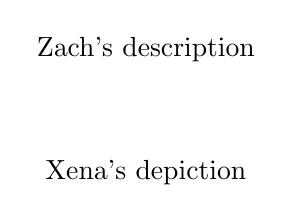
\begin{tikzpicture}
                \node (x_tilde) {Xena's depiction};
                \node[above=of x_tilde] (z) {Zach's description};
            \end{tikzpicture}
        };
        \draw[->] (x) -- (z_hat);
        \draw[->] (z) -- (x_tilde);
        \draw[->] (q) -- (discriminator);
        \draw[->] (p) -- (discriminator);
    \end{tikzpicture}
    \caption{\label{fig:model_story} A Circle of Infinite Painters' view of the
        ALI game.}
\end{figure}

The Circle of Infinite Painters is a very prolific artistic group. Very little
is known about the Circle, but what we do know is that it is composed of two
very brilliant artists. It has produced new paintings almost daily for more than
twenty years, each one more beautiful than the others. Not only are the
paintings exquisite, but their title and description is by itself a literary
masterpiece.

However, some scholars believe that things might not be as they appear: certain
discrepancies in the Circle's body of work hints at the Circle being composed of
more than one artistic duo. This is what Joseph Discriminator, art critique and
world expert on the Circle, believes. He's recently been working intensively on
the subject. Without knowing it, he's right: the Circle is not one, but two
artistic duos.

Xavier and Zach Prior form the creative component of the group. Xavier is a
painter and can, in one hour and starting from nothing, produce a painting that
would make any great painter jealous. Impossible however for him to explain
what he's done: he works by intuition alone. Zach is an author and his literary
talent equals Xavier's artistic talent. His verb is such that the scenes he
describes could just as well be real.

By themselves, the Prior brothers cannot collaborate: Xavier can't paint
anything from a description and Zach is bored to death with the idea of
describing anything that does not come out of his head. This is why the Prior
brothers depend on the Conditional sisters so much.

Zelda Conditional has an innate descriptive talent: she can examine a painting
and describe it so well that the original would seem like an imitation. Xena
Conditional has a technical mastery of painting that allows her to recreate
everything that's described to her in the most minute details. However, their
creativity is inversely proportional to their talent: by themselves, they cannot
produce anything of interest.

As such, the four members of the Circle work in pairs. What Xavier paints, Zelda
describes, and what Zach describes, Xena paints. They all work together to
fulfill the same vision of a unified Circle of Infinite Painters, a whole greater
than the sum of its parts.

This is why Joseph Discriminator's observations bother them so much. Secretly,
the Circle put Mr. Discriminator under surveillance. Whatever new observation
he's made, they know right away and work on attenuating the differences to
maintain the illusion of a Circle of Infinite Painters made of a single artistic
duo.

Will the Circle reach this ideal, or will it be unmasked by Mr. Discriminator?
}{}

\end{document}
